\documentclass[conference,onecolumn]{IEEEtran}
\IEEEoverridecommandlockouts

\usepackage{cite}
\usepackage{amsmath,amssymb,amsfonts}
\usepackage{graphicx}
\usepackage{textcomp}
\usepackage{xcolor}
\usepackage{booktabs}
\usepackage{tabularx}
\usepackage{array}
\usepackage{float}
\usepackage{url}

\Urlmuskip=0mu plus 2mu\relax
\def\UrlBreaks{\do\/\do-\do\_\do\.\do\?\do\=\do\&}
\emergencystretch=2em

\graphicspath{{../results/presentation/}{../results/}}
\newcolumntype{Y}{>{\raggedright\arraybackslash}X}
\newcommand{\pjbit}{pJ/bit}
\newcommand{\tbps}{Tb/s}
\newcommand{\code}[1]{\texttt{#1}}
\newcommand{\figref}[1]{Fig.~\ref{#1}}
\newcommand{\tabref}[1]{Table~\ref{#1}}

\def\BibTeX{{\rm B\kern-.05em{\sc i\kern-.025em b}\kern-.08em
    T\kern-.1667em\lower.7ex\hbox{E}\kern-.125emX}}

\begin{document}

\title{Topology-Aware Mapping for Photonic Interconnects in TPU-Class LLM Accelerators}

\author{
\IEEEauthorblockN{Pranav Sitaraman}
\IEEEauthorblockA{sitaraman.pranav@gmail.com}
\and
\IEEEauthorblockN{Simone Surdi}
\IEEEauthorblockA{simonesurdi@gmail.com}
}

\maketitle

\section{Project Overview}

This project is based on Project 12, ``Evaluate a New Technology,'' using the
AccelForge cluster-mapping example as the starting point. The technology we will
study is co-packaged photonic interconnect, with Lightmatter Passage used as a
concrete public reference point. The question is not just whether optical links
save link energy but also whether a photonic fabric
changes what a good accelerator mapping looks like.

That distinction matters for modern LLM systems. A TPU pod exposes a large
software-visible pool of HBM, but physically that memory is distributed across
many chips. Ironwood/TPU7x, for example, is publicly described as a 9216-chip
pod with 192 GiB HBM and 1200 GB/s bidirectional ICI per chip
\cite{tpu7x,ironwood-blog}. If the compiler treats remote memory as expensive,
it will tend to keep data local, replicate state, and use familiar collectives. If remote reads, cache fills, and multicast become cheap enough,
the compiler may instead prefer shared weight broadcasts, pooled HBM, or
different expert-placement choices. That is the design space this project
models.

The central hypothesis is that photonics will help most when traffic either
leaves the local HBM bank or fans out to many chips. Local node-to-node traffic
should improve only modestly, because an electrical torus is already well
matched to nearest-neighbor exchange. Shared-state multicast, KV-cache traffic,
remote weight refill, and MoE routing should improve much more. We also expect
inference to benefit more than training since inference has exposed network stages while training becomes compute dominated once gradient and expert traffic are
reduced.

Our current work already gives useful pilot evidence for this proposal. In
a 16-node AccelForge study, EVK100-style optical links reduce energy by up to
72.21\% and latency by up to 97.57\% for remote-memory and multicast traffic.
On a 64-chip TPU-cube model, an M1000-style switched optical fabric reduces
network energy by up to 99.91\% for shared-weight multicast. More importantly,
the optimal distributed mapping changes in 5 of 16 tested cases, which is the
first sign that this is not just a lower-\pjbit{} substitution.

\section{Technical Contributions}

Existing accelerator tools are good at modeling local compute, SRAM/HBM action
counts, and loop mappings, but they do not usually make the network topology a
first-class part of the mapper. AccelForge follows this pattern since it can model a
logical memory hierarchy but does not natively know whether that logical
memory is backed by a 2-D mesh, 3-D torus, advanced chiplet fabric, or optical
crossbar. Separately, public material from Google and Lightmatter gives
technology facts about TPU systems and photonic interconnects
\cite{lightmatter-passage,lightmatter-m1000,tpu7x,hotchips-ironwood}, but those
facts are not tied to a mapper-visible cost model.

Our contribution is to connect these pieces in a way that the mapper and the
compiler-visible dataflow can use. The implementation will have the following four parts.
\begin{itemize}
    \item A topology model for ring, mesh, torus, crossbar, and switched
    optical fabrics. The model accounts for hop count, contention, bandwidth,
    link energy, router latency, and multicast support.
    \item A logical cluster-memory level in the AccelForge architecture. After
    each mapper run, logical-memory reads and writes are converted into network
    traffic, the network cost is added back into the memory level, and the
    mapper is re-run to a fixed point.
    \item A distributed mapping selector that compares node-to-node exchange,
    node-to-DRAM remote reads, and shared-DRAM multicast. This is where the
    project tests whether photonics changes the best communication pattern.
    \item A higher-level compiler/dataflow model for choices that AccelForge's
    inner tile mapper does not express directly like potentially XLA-style collectives,
    photonic multicast cache fills, remote pooled-HBM streaming, and MoE
    locality routing.
\end{itemize}

\begin{table}[H]
\centering
\caption{Interconnect points used in the model.}
\label{tab:tech}
\footnotesize
\begin{tabularx}{\linewidth}{l r r c Y}
\toprule
Technology & BW & Energy & Multicast & Why it is included \\
\midrule
Electrical ICI & 0.8~\tbps{} & 10.0~\pjbit{} & No & TPU-like electrical baseline. \\
Advanced chiplet & 3.5~\tbps{} & 6.0~\pjbit{} & No & Stronger packaging baseline requested for comparison. \\
Lightmatter EVK100 & 3.2~\tbps{} & 1.9~\pjbit{} & Yes & Main conservative photonic proposal point. \\
Lightmatter L200/L200X & 16--32~\tbps{} & 4.5--4.8~\pjbit{} & Yes & Higher-bandwidth photonic fabric sweep. \\
Lightmatter M1000 & 57.3~\tbps{} & 2.3~\pjbit{} & Yes & Switched optical fabric used for the full-system study. \\
\bottomrule
\end{tabularx}
\end{table}

The project has a few important limitations. The Lightmatter numbers are public
headline values, so the goal is to model the architecture as a whole rather than a particular product. Furthermore, optical multicast is modeled
optimistically as one logical broadcast. Finally, Google has not published
Gemini 3 or Gemini 3.1 parameter counts. For that reason, the superpod
experiments use explicit dense, sparse-MoE, and long-context proxy workloads
that mirror frontier LLMs trained on Google's TPUs rather than their own ground-truth private architectures.

\section{Evaluation}

The evaluation holds the accelerator compute and memory hierarchy fixed unless
the experiment explicitly says otherwise. The baseline is an electrical
TPU-like fabric. The main photonic comparison is Lightmatter-style EVK100 or
M1000, and the stronger non-photonic comparison is the advanced chiplet model
with 3.5~\tbps{} one-way bandwidth and 6~\pjbit{} per hop. This keeps the
analysis focused to how the energy, latency,
scaling, and mapping choices respond to interconnect changes.

\begin{table}[H]
\centering
\caption{Initial measurements that motivate the final evaluation.}
\label{tab:pilot}
\footnotesize
\begin{tabularx}{\linewidth}{l r Y}
\toprule
Measurement & Value & Interpretation \\
\midrule
Best 16-node energy reduction & 72.21\% & EVK100 crossbar helps most for shared-DRAM multicast. \\
Best 16-node latency reduction & 97.57\% & Network-aware fixed point nearly removes the exposed KV-attention multicast delay. \\
Best TPU-cube network energy reduction & 99.91\% & M1000 switched fabric avoids repeated torus fanout for shared weights. \\
Changed distributed mappings & 5/16 cases & Photonics makes shared-DRAM multicast preferable for several prefill cases. \\
Best compiler-strategy energy gain & 67.75\% & Remote pooled-HBM streaming becomes attractive on M1000. \\
Best chiplet-relative energy reduction & 99.85\% & M1000 still beats the stronger chiplet baseline for shared-state multicast. \\
Best superpod inference speedup & 14.50\(\times\) & Long-context proxy inference benefits from topology plus compiler changes. \\
Best superpod training speedup & 1.43\(\times\) & Training improves, but becomes compute dominated. \\
\bottomrule
\end{tabularx}
\end{table}

\subsection{Experiment 1: topology-aware AccelForge mapping}

The first experiment compares an electrical 4\(\times\)4 mesh with an EVK100
optical crossbar on 16 nodes, then repeats the idea on a 4\(\times\)4\(\times\)4
TPU cube. The workloads are GEMM-shaped LLM kernels: decode MLP, KV attention,
prefill projection, long-context prefill, MoE dispatch, and training
weight-gradient accumulation. The communication choices are node-to-node,
node-to-DRAM, and shared-DRAM multicast.

This experiment emphasizes the placement cost of memory traffic. We will report total energy, total latency,
network energy share, and whether the final mapping or distributed
communication choice changes. The expected trend is that multicast and remote
memory improve far more than local exchange.

\begin{figure}[H]
    \centering
    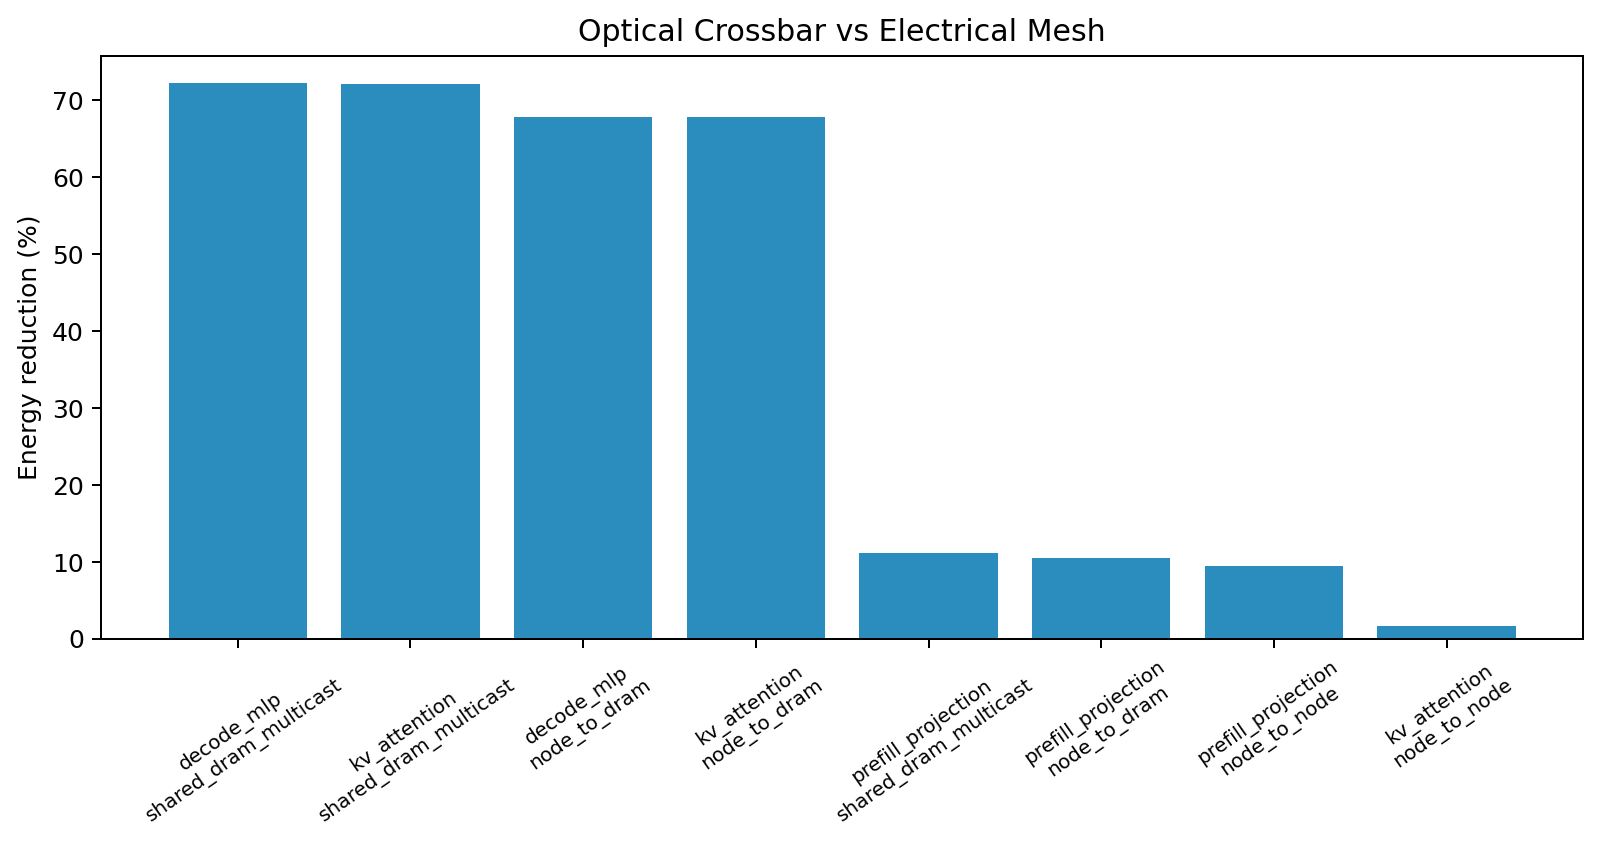
\includegraphics[width=0.6\linewidth]{01_cluster_reductions.png}
    \caption{Preliminary 16-node results. Optical links help most when traffic
    leaves local memory or fans out to many nodes.}
    \label{fig:cluster}
\end{figure}

\subsection{Experiment 2: scaling, topology, and stronger baselines}

The second experiment analyzes whether the result survives a better baseline. In
addition to the electrical TPU torus, we include an advanced chiplet model with
3.5~\tbps{} links and 6~\pjbit{} per hop. The system size is swept from one
64-chip cube toward the 9216-chip superpod scale. The main metrics are energy,
latency, and the log-log scaling exponent of per-chip cost.

The expected result is not that every photonic topology wins everywhere. A
photonic torus can still inherit torus hop growth. The stronger claim is that a
switched optical fabric changes the scaling law for global traffic by keeping
logical hop count and multicast fanout nearly flat.

\begin{figure}[H]
    \centering
    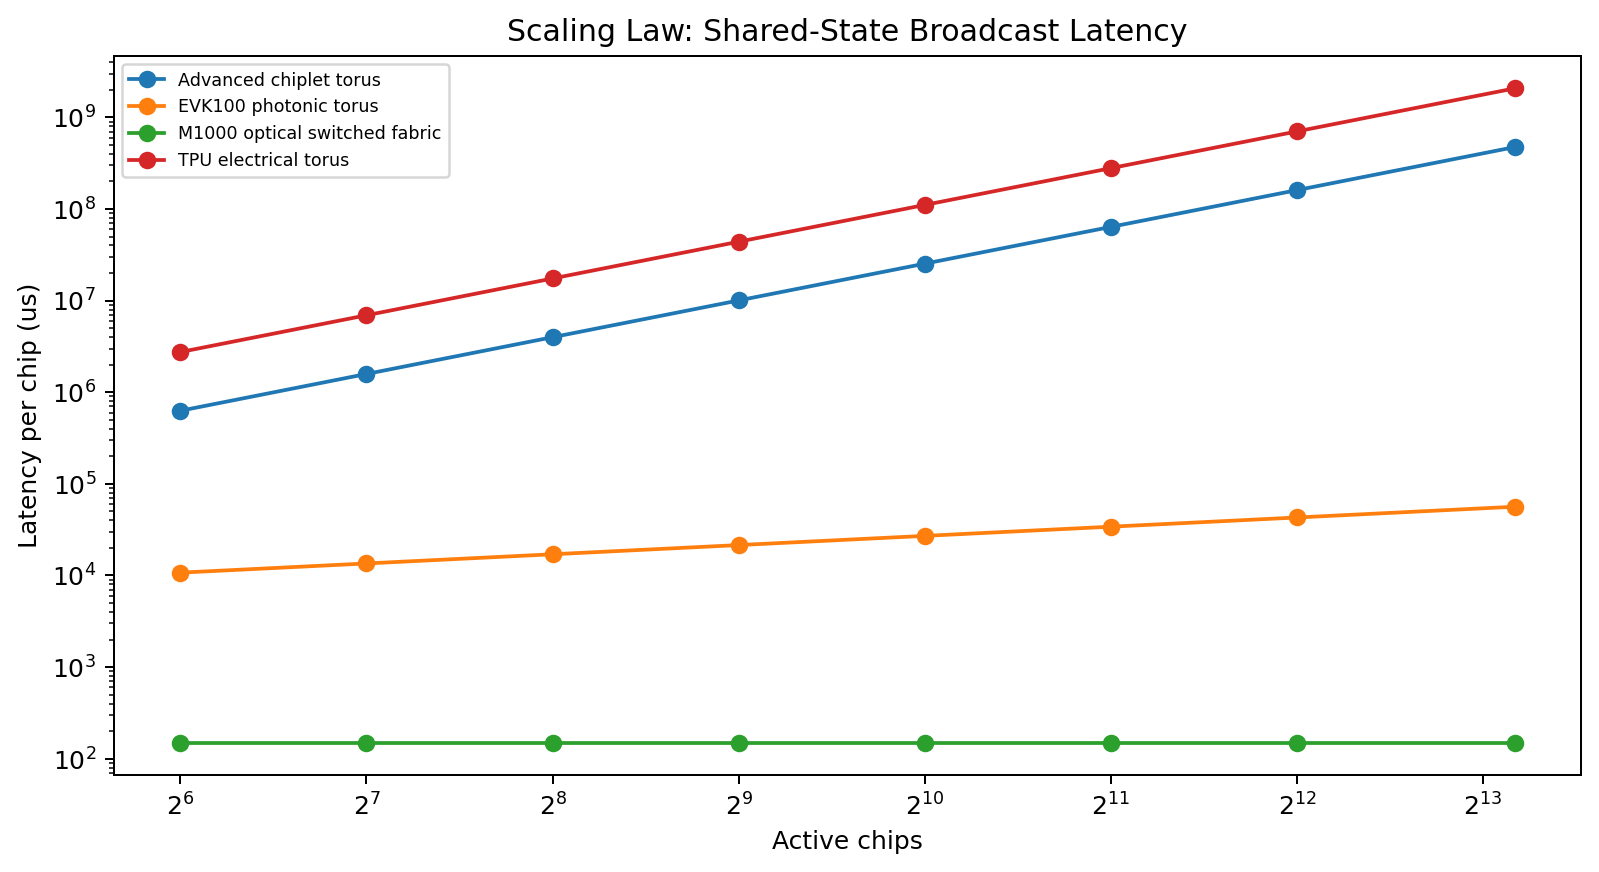
\includegraphics[width=0.6\linewidth]{05_scaling_laws.png}
    \caption{Preliminary scaling sweep. Switched photonics stays nearly flat
    for all-to-all and shared multicast, while torus and chiplet fabrics
    accumulate hop and contention cost.}
    \label{fig:scaling}
\end{figure}

\subsection{Experiment 3: compiler-visible dataflow and full-superpod impact}

The third experiment moves above the inner tile mapper. It evaluates whether
photonic interconnect should change compiler-visible choices such as
sharding, cache fill, remote HBM access, and expert routing. This is important
because the current AccelForge tile mapping can remain stable even while the
best distributed dataflow changes.

For the final system study, we model public frontier proxy workloads on a
9216-chip Ironwood/TPU7x pod: a dense Flash-class proxy, a sparse MoE
Pro-class proxy, and a long-context Deep Think-class proxy. The model will be divided into stages like prefill, decode KV attention, weight/expert refill, MoE
dispatch/combine, training forward/backward, gradient synchronization, and
optimizer traffic. The output will be an ablation ladder showing how much of the gain is expected to come from the chiplet baseline, photonic torus, switched topology, multicast
cache fills, remote HBM, MoE locality, and the full photonic compiler stack.

\begin{figure}[H]
    \centering
    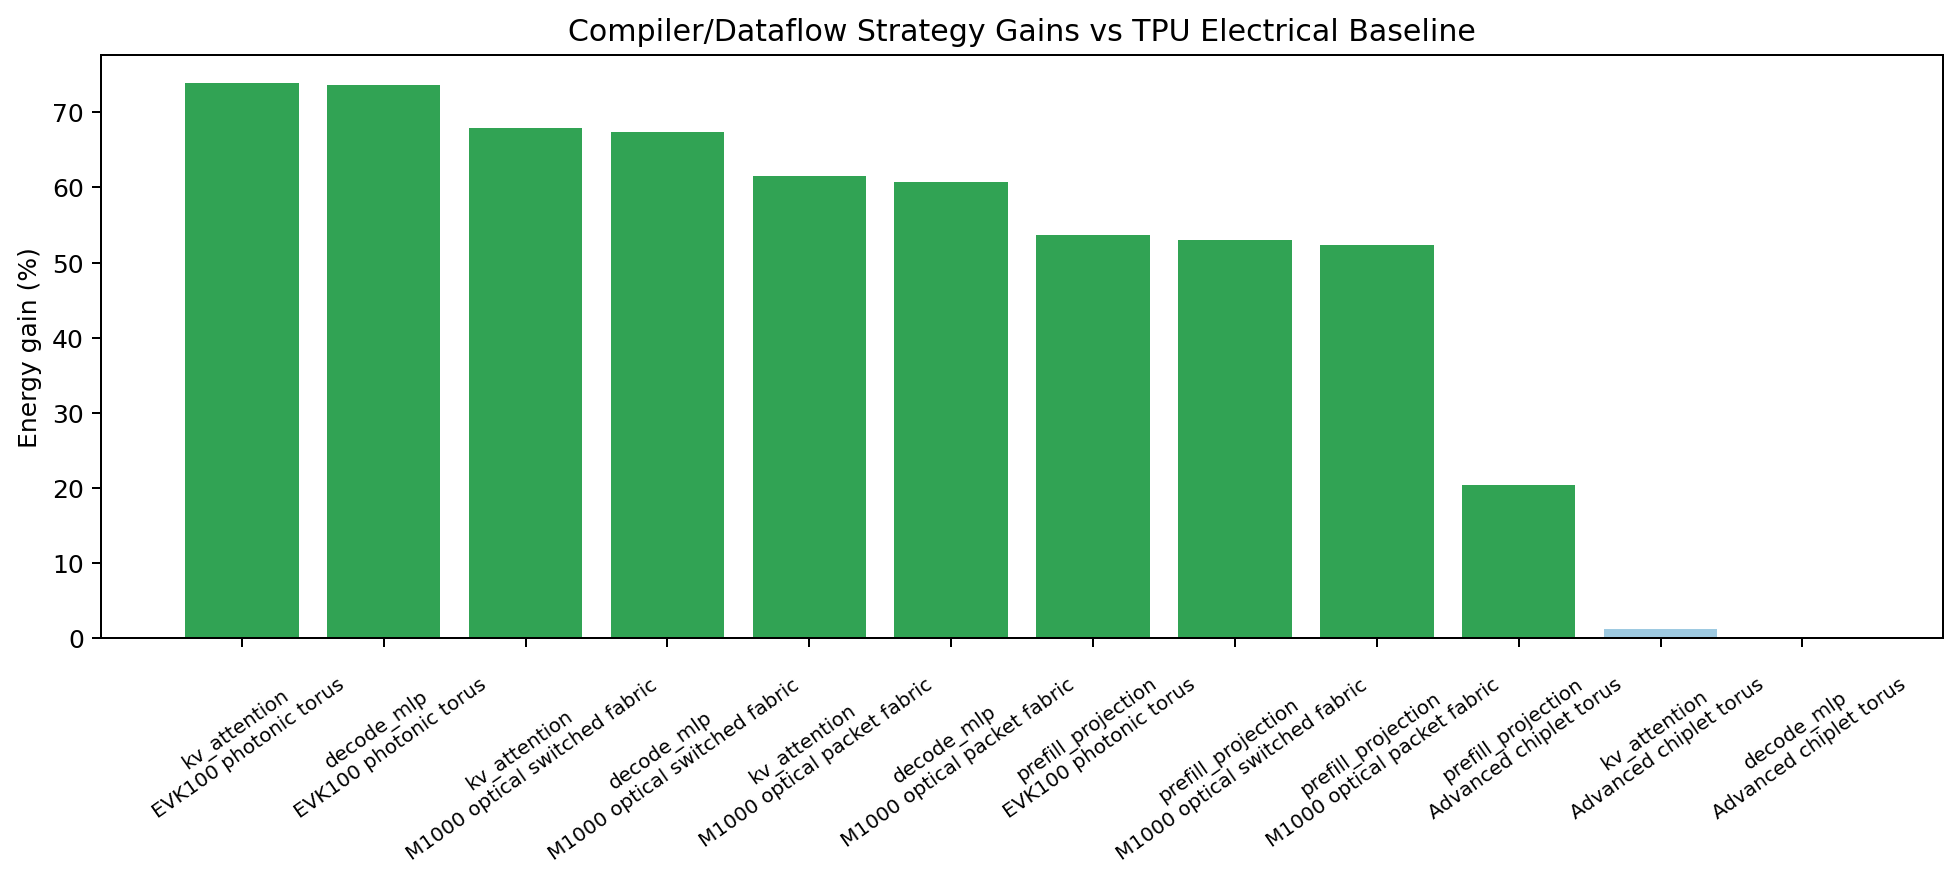
\includegraphics[width=0.7\linewidth]{04_compiler_strategy_choices.png}
    \caption{Preliminary compiler/dataflow results. The green bars mark cases
    where the best compiler-visible strategy changes under photonics.}
    \label{fig:compiler}
\end{figure}

\begin{figure}[H]
    \centering
    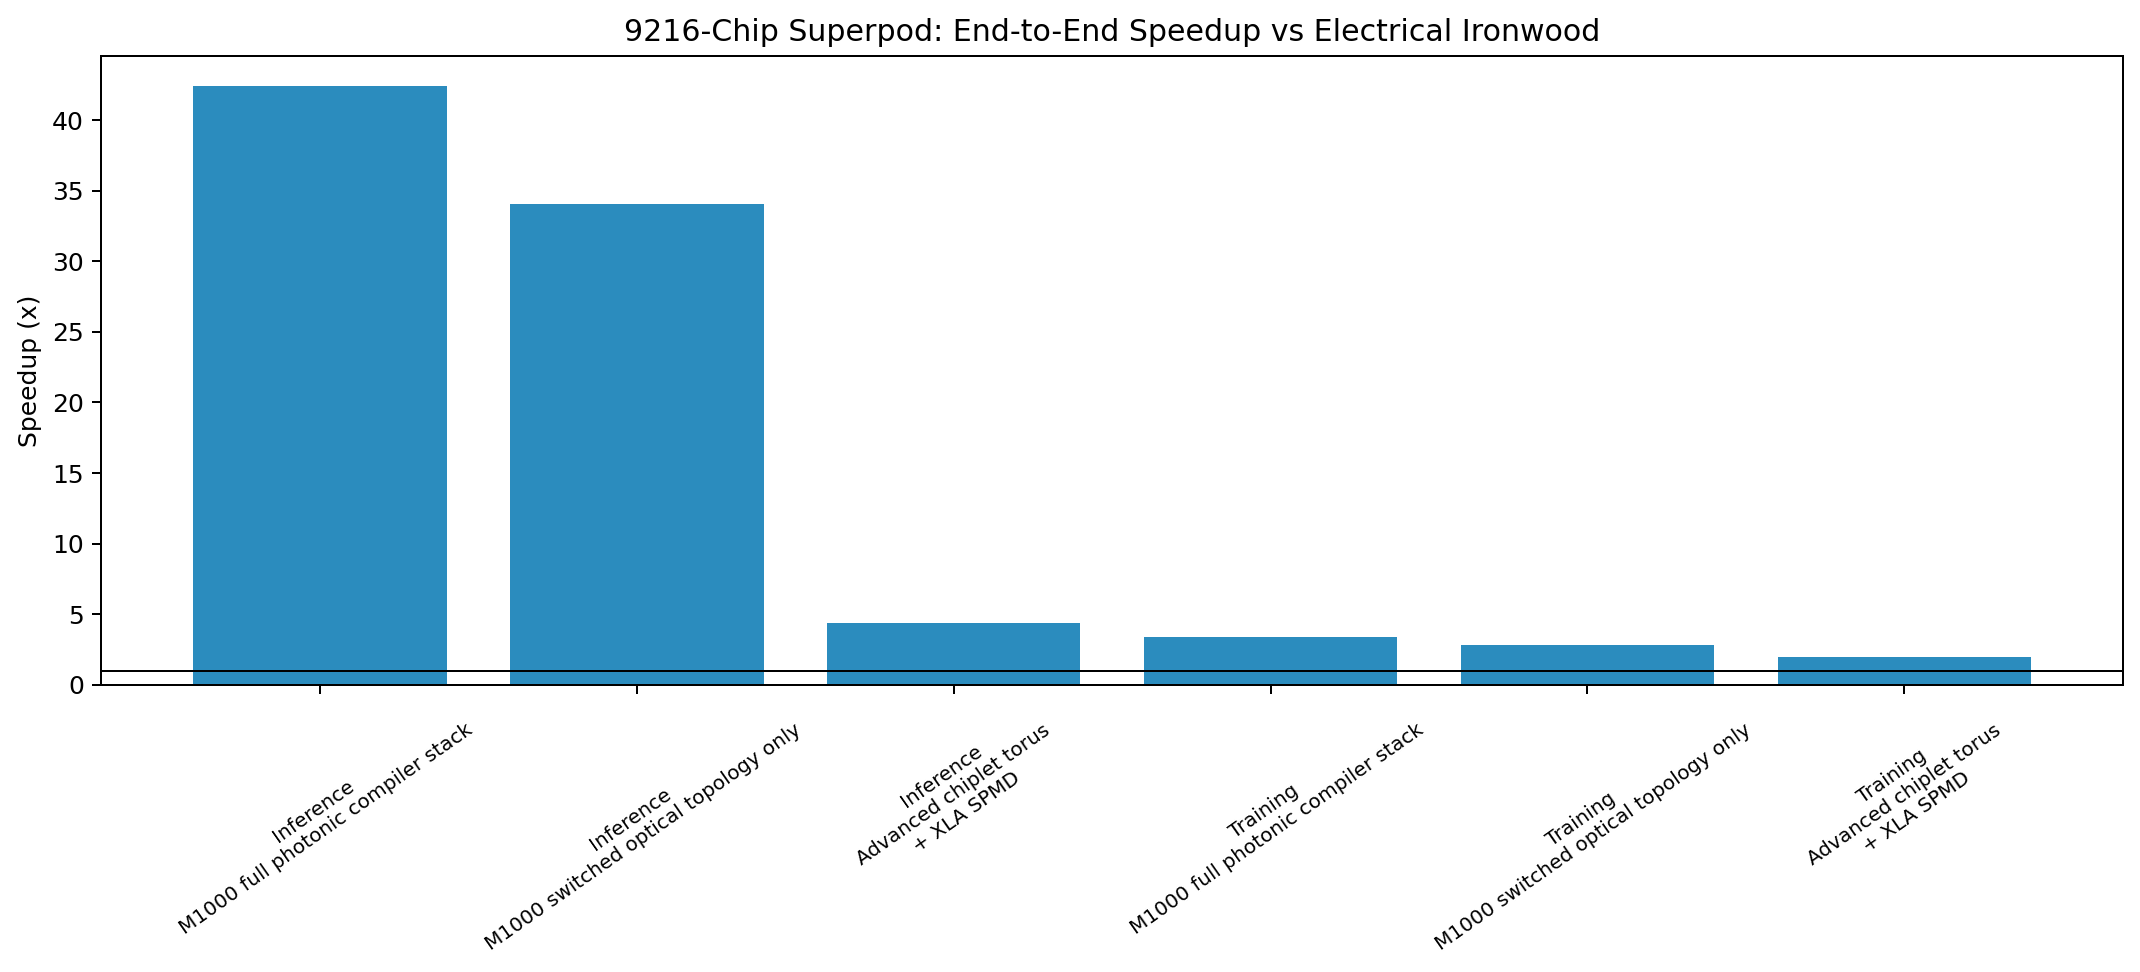
\includegraphics[width=0.7\linewidth]{07_superpod_end_to_end_speedups.png}
    \caption{Preliminary 9216-chip proxy results. Inference benefits much more
    than training because decode, cache, and routing traffic are network
    exposed.}
    \label{fig:superpod}
\end{figure}

The main results we expect to defend are that photonics should reduce energy and latency directly and also induce new mappings such as multicast instead
of repeated unicast, pooled remote memory instead of strict local replication,
and topology-aware compiler choices instead of a fixed default.

\section{Timeline and Work Distribution}

The project implementation is sufficiently in progress to support the preconditions and hypotheses of the proposal, so the
remaining work is running full-scale experiments, validation, and tackling further stretch goals before organizing the work into a complete and cohesive presentation. The plan is as follows.

\begin{table}[H]
\centering
\caption{Work plan and current status.}
\label{tab:timeline}
\footnotesize
\begin{tabularx}{\linewidth}{l l Y}
\toprule
Milestone & Status & Deliverable \\
\midrule
M1: topology model and logical memory & Complete & Ring/mesh/torus/crossbar models, traffic accounting, and logical cluster memory in AccelForge. \\
M2: iterative network-aware mapper & Complete & Fixed-point mapper loop, convergence traces, energy breakdowns, and cluster CSVs. \\
M3: improved topology proposal & In progress & EVK100 optical crossbar and TPU-cube photonic alternatives. \\
Mapping and compiler study & In progress & Distributed mapping selector, compiler/dataflow strategy model, and mapping-change tables. \\
Scaling and chiplet comparison & In progress & 64-to-9216-chip scaling sweeps and advanced chiplet baseline. \\
Final writeup and presentation & Not started & Condensed figures, final report text, validation notes, and slide-ready summary. \\
\bottomrule
\end{tabularx}
\end{table}

With the project split across the two of us, Simone will own the AccelForge/network
model while Pranav will own the compiler/superpod analysis, with the codebase organized around that boundary. The plan is to finish the currently in-progress tasks at least a week before the presentation deadline and to spend the remaining time polishing up the final project deliverables.

\begin{thebibliography}{99}

\bibitem{lightmatter-passage}
Lightmatter, ``Passage product family,'' viewed Apr. 2026.
\url{https://lightmatter.co/products/passage/}

\bibitem{lightmatter-m1000}
Lightmatter, ``Passage M1000 EVK,'' viewed Apr. 2026.
\url{https://lightmatter.co/products/passage-m1000-evk/}

\bibitem{lightmatter-l200}
Lightmatter, ``Passage L200,'' viewed Apr. 2026.
\url{https://lightmatter.co/products/l200/}

\bibitem{lightmatter-sc25}
Lightmatter, ``Bob Turner SC25 Passage EVK50 resource,'' Dec. 2025.
\url{https://lightmatter.co/resource/bobturnersc25/}

\bibitem{tpu7x}
Google Cloud, ``Cloud TPU7x,'' last updated Apr. 15, 2026.
\url{https://docs.cloud.google.com/tpu/docs/tpu7x}

\bibitem{ironwood-blog}
Google Cloud, ``Inside the Ironwood TPU co-designed AI stack,'' viewed Apr. 2026.
\url{https://cloud.google.com/blog/products/compute/inside-the-ironwood-tpu-codesigned-ai-stack/}

\bibitem{hotchips-ironwood}
P. Kanwar, ``TPU Rack Scale Systems,'' Hot Chips 2025 tutorial, Aug. 2025.
\url{https://hc2025.hotchips.org/assets/program/tutorials/HC2025.T1DCRacks.S7.Pankaj.pdf}

\bibitem{xla-spmd}
PyTorch/XLA, ``SPMD user guide,'' viewed Apr. 2026.
\url{https://docs.pytorch.org/xla/master/spmd.html}

\bibitem{gemini3}
Google, ``Introducing Gemini 3,'' Nov. 2025.
\url{https://blog.google/products-and-platforms/products/gemini/gemini-3/}

\bibitem{gemini3deepthink}
Google, ``Gemini 3 Deep Think,'' Feb. 2026.
\url{https://blog.google/innovation-and-ai/models-and-research/gemini-models/gemini-3-deep-think/}

\end{thebibliography}

\end{document}
